\par Cette partie présente la conception préliminaire qui a été réalisée. \\

\par Le diagramme en figure 1 représente les différentes briques logicielles de la chaîne de traitement mise en place pour déterminer les stances de tweets.

\subsection{Diagramme du flux de traitement des données}
\begin{figure}[h!]
	\centerline{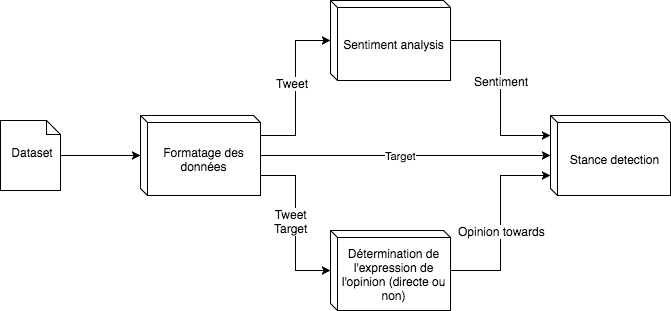
\includegraphics[scale=0.8]{img/diagramme_flux_traitement.png}}
	\caption{Diagramme de flux de traitement des données}
	\label{flux_diagram}
\end{figure}
\newpage


\par Durant ce projet plusieurs technique de machine learning ont été nécessaire, en figure 2 il est possible de trouver un schéma du processus d'apprentissage. \\

\subsection {Diagramme de la couche machine learning}
\begin{figure}[h!]
	\centerline{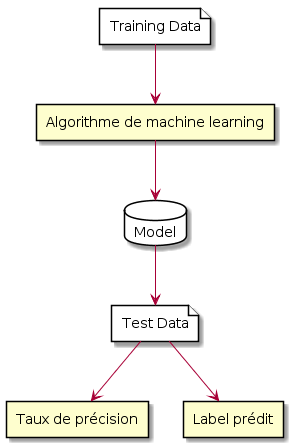
\includegraphics[scale=0.8]{img/diagramme_machine_learning.png}}
	\caption{Diagramme des méthodes d'apprentissage}
\end{figure}
\newpage


\subsection {Conception Sentiment Analysis}

\par Concernant la brique Sentiment Analysis, plusieurs méthodes sont possibles, en figure 3 vous pouvez retrouver un diagramme détaillant plusieurs méthodes pour la détection de sentiment de tweet et en figure 4 la conception pour une méthode en particulier. \\


\begin{figure}[h!]
	\centerline{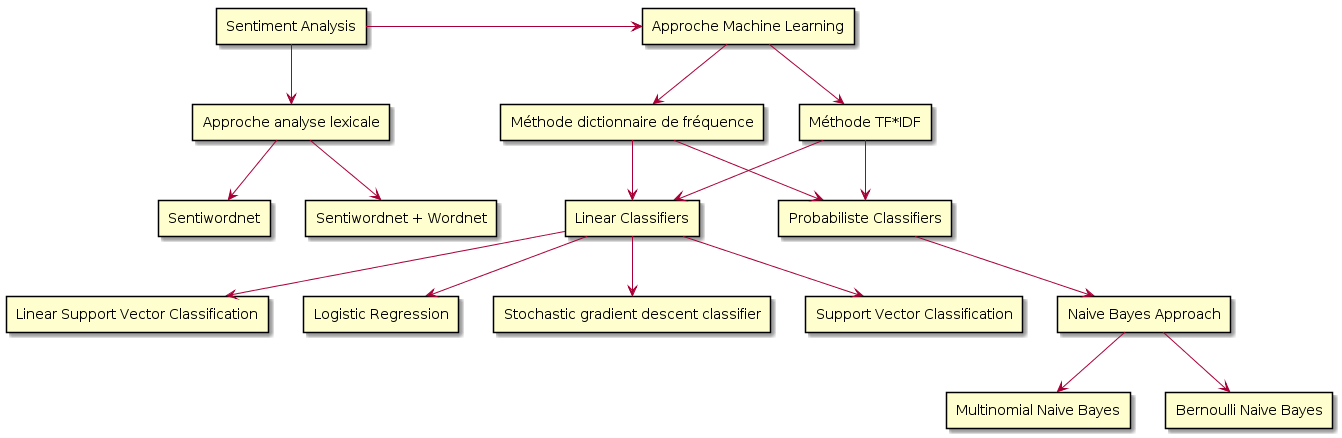
\includegraphics[scale=0.4]{img/diagramme_sentiment_analysis.png}}
	\caption{Diagramme général de la brique Sentiment Analysis}
\end{figure}


\begin{figure}[h!]
	\centerline{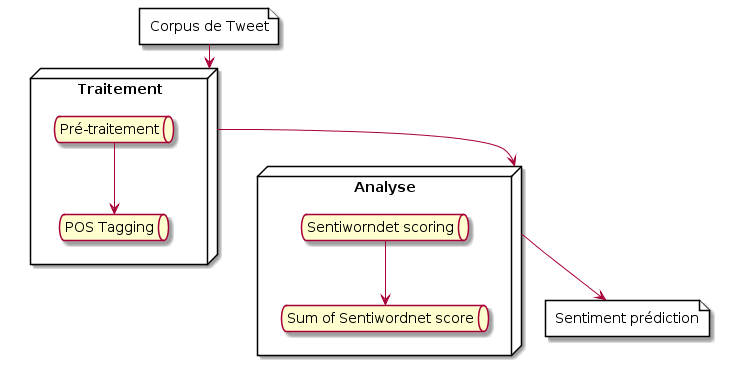
\includegraphics[scale=0.6]{img/diagramme_sentiwordnet.png}}
	\caption{Diagramme de la méthode de détection de sentiment par sentiwordnet}
\end{figure}
